% Section 1 - Actions
% Roberto Masocco <roberto.masocco@uniroma2.it>
% May 2, 2026

% ### Actions ###
\section{Actions}
\graphicspath{{figs/section1/}}

% --- Limitations of services ---
\begin{frame}{Limitations of services}
  \justifying
  The third paradigm exists because services rely on the following \textbg{restrictive assumptions}.\\
  \medskip
  \begin{alertblock}{Services implementation assumptions}
    \justifying
    \begin{itemize}
      \item Since the client may block for the entire duration of the request processing, \textbr{server computations should be short and always produce some result} (\emph{e.g.}, even an error must be a result if necessary, but \textbr{we} have to encode it, the API does not provide it).
      \item Once a service is called, \textbr{the processing of the request may never be interrupted}.
    \end{itemize}
    \medskip
    In short, service-based communications are \textbr{stateless} as the topic-based ones.
  \end{alertblock}
  \medskip
  These make \textbg{completely unfeasible} operations that \textbg{must be requested} and \textbg{take a long time} (for CPUs!).\\
  Think of real stuff such as \textbg{movement}, \textbg{navigation}...
\end{frame}

% --- ROS 2 actions ---
\begin{frame}{ROS 2 actions}{Full client-server paradigm}
  \justifying
  Built on services and message topics, they \textbg{decouple operations from the middleware API}, thanks to three concepts that model the \textbg{three stages of an operation}.
  \begin{enumerate}
    \item \textbg{Goal}: the request of the operation to be executed, complete of input data.
    \item \textbg{Feedback}: intermediate results and information about the ongoing processing.
    \item \textbg{Result}: the final result of the requested operation, with output data.
  \end{enumerate}
  \bigskip
  Their implementation is still a bit cumbersome because of the \textbg{many different data types} (classes) involved, as well as many \textbg{API inconsistencies}.\\
  It is found in the \href{https://github.com/ros2/rclcpp/tree/jazzy/rclcpp_action}{\color{blue}{\underline{\texttt{rclcpp\_action}}}} and \href{https://github.com/ros2/rclpy/tree/jazzy/rclpy/rclpy/action}{\color{blue}{\underline{\texttt{rclpy action}}}} libraries.\\
  \bigskip
  They are \textbg{extensively used to implement robot navigation and movement}, and many more complex real-world operations, providing a \textbg{software abstraction} for them.
\end{frame}
\begin{frame}{ROS 2 actions}{Full client-server paradigm}
  \begin{figure}
    \centering
    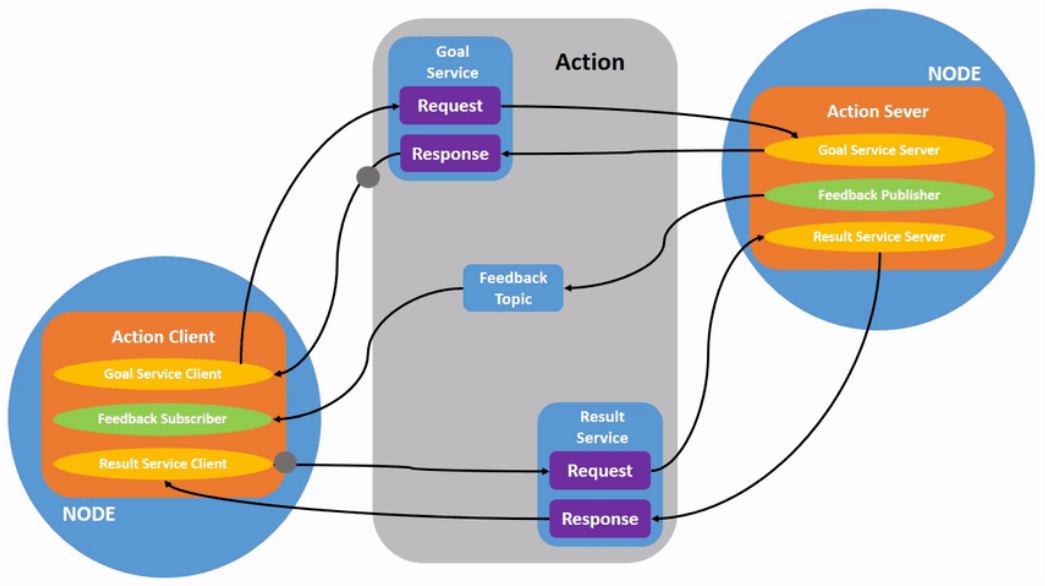
\includegraphics[scale=.37]{ros2Act.png}
    \caption{Example of an action \emph{server} and \emph{client}.}
    \label{fig:ros2Act}
  \end{figure}
\end{frame}
\begin{frame}{ROS 2 actions}{The goal state machine}
  \begin{figure}
    \centering
    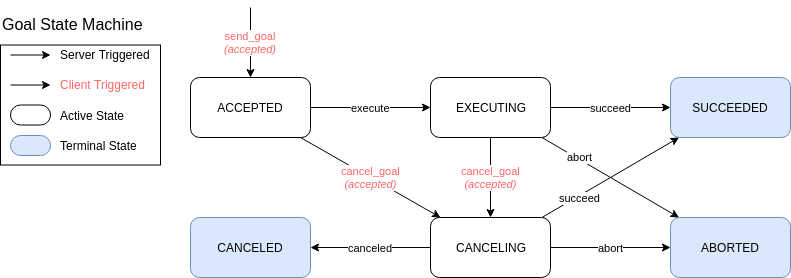
\includegraphics[width=\textwidth]{goalStateMachine.png}
    \caption{State machine\footnote{\href{http://design.ros2.org/articles/actions.html}{\color{blue}\underline{Actions - ROS 2 Design}}} of an action goal, implemented and managed internally by ROS 2.}
    \label{fig:goalStateMachine}
  \end{figure}
\end{frame}
\begin{frame}{ROS 2 actions}{Communication overview}
  \justifying
  In ROS 2 applications, the \textbg{client} requests the completion of some \textbg{goal} to the \textbg{server}.\\
  The middleware offers \textbg{API to share and update the state of the goal among the two}.
  \medskip
  \begin{enumerate}
    \item The \textbg{client} sends a \textbg{goal service request} to the server.
    \item The \textbg{server} may \textbg{accept} or \textbg{reject} the goal request.
    \item Server computations are usually started when the goal is \textbg{executed}: the middleware only keeps track the state of the goal, the rest is up to the developer.
    \item The \textbg{client may cancel} the goal request; the \textbg{server may abort} the goal request; intermediate results and information, if any, are published by the server on the \textbg{feedback topic}.
    \item The \textbg{client} asks the server for the final result over the \textbg{result service}.
  \end{enumerate}
\end{frame}
\begin{frame}{ROS 2 actions}{CLI introspection tools}
  \justifying
  The main command is \texttt{ros2 action} with the following verbs.
  \begin{itemize}
    \item \texttt{list} Lists all active actions.
    \item \texttt{info} Prints information about an action.
    \item \texttt{send\_goal} Sends a goal request to an action server and prints the result; with \texttt{-f} prints also feedback messages.
  \end{itemize}
\end{frame}
\begin{frame}{ROS 2 actions}{Coding hints for servers and clients}
  \begin{block}{Servers}
    \justifying
    Goal requests are handled with \textbf{callbacks}, while computations can be handled freely (usually done in \textbf{separate threads}).\\
    \textbf{Cancellation requests} are handled with \textbf{callbacks} and can be \textbf{polled} during the computation.\\
    When done, the goal must be marked as \textbf{succeeded} or \textbf{aborted}.
  \end{block}
  \begin{block}{Clients}
    \justifying
    Similarly to services, much is done with \textbf{\texttt{future} objects}, but \textbf{callbacks may be defined} to handle \textbf{goal}, \textbf{result} and \textbf{cancellation responses}, as well as \textbf{feedbacks}.
  \end{block}
  \begin{block}{}
    \centering
    Handling all possible scenarios for a goal results in the \textbf{longest and most complicated code that a ROS 2 application may ever require}. {\Large\smiley{}}
  \end{block}
\end{frame}

% --- Interface files - Actions ---
\begin{frame}[fragile]{Interface files}{Actions}
  \justifying
  Combine \textbg{three messages} in a single interface file, separated by \texttt{-{}-{}-}.\\
  Action file names end with \texttt{.action}.
  \begin{columns}
    \column{.9\textwidth}
    \begin{lstlisting}[language=ros2msg, caption=Definition of the \texttt{ros2\_examples\_interfaces/action/Fibonacci} action.]
# GOAL
int32 order
---
# RESULT
int32[] sequence
---
# FEEDBACK
int32[] partial_sequence
    \end{lstlisting}
  \end{columns}
\end{frame}

% --- Example - Fibonacci computer ---
\begin{frame}{Example}{Fibonacci computer}
  \justifying
  \begin{block}{}
    \centering
    Now go have a look at the \href{https://github.com/IntelligentSystemsLabUTV/ros2-examples/tree/jazzy/src/cpp/actions_example_cpp}{\color{blue}\underline{\texttt{ros2-examples/src/cpp/actions\_example\_cpp}}} package!
  \end{block}
  \bigskip
  If you are curious, the \href{https://github.com/IntelligentSystemsLabUTV/ros2-examples/tree/jazzy/src/cpp/advanced/complete_actions_cpp}{\color{blue}\underline{\texttt{ros2-examples/src/cpp/advanced/complete\_actions\_cpp}}} package implements the complete goal state machine using a multithreaded executor.
\end{frame}
